\documentclass{article}
\usepackage[utf8]{inputenc}
\usepackage[margin=1in]{geometry}
\usepackage{float}
\usepackage{tikz}
\usepackage{tikz-qtree}

\title{Data Structures: Problem Set 4}
\author{Jackie Luo}
\date{April 19, 2015}

\begin{document}
\maketitle

\section{Theory}

\subsection{}
a.
\newline
\begin{figure}[H]
\centering
\begin{tikzpicture}
\Tree [.3 ]
\end{tikzpicture}
\caption{[3]}
\end{figure}

\begin{figure}[H]
\centering
\begin{tikzpicture}
\Tree [.3 9 \edge[draw=none]; {} ]
\end{tikzpicture}
\caption{[3, 9]}
\end{figure}

\begin{figure}[H]
\centering
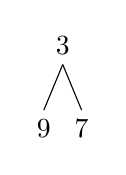
\begin{tikzpicture}
\Tree [.3 9 7 ]
\end{tikzpicture}
\caption{[3, 9, 7]}
\end{figure}

\begin{figure}[H]
\centering
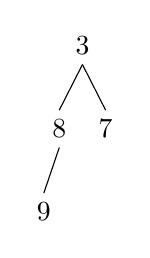
\begin{tikzpicture}
\Tree [.3 [.8 9 \edge[draw=none]; {} ] 7 ]
\end{tikzpicture}
\caption{[3, 8, 7, 9]}
\end{figure}

\begin{figure}[H]
\centering
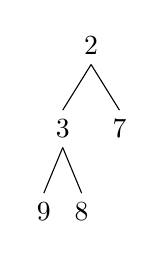
\begin{tikzpicture}
\Tree [.2 [.3 9 8 ] 7 ]
\end{tikzpicture}
\caption{[2, 3, 7, 9, 8]}
\end{figure}

\begin{figure}[H]
\centering
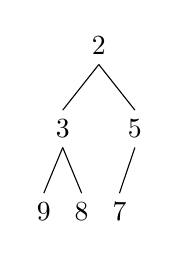
\begin{tikzpicture}
\Tree [.2 [.3 9 8 ] [.5 7 \edge[draw=none]; {} ] ]
\end{tikzpicture}
\caption{[2, 3, 5, 9, 8, 7]}
\end{figure}

\begin{figure}[H]
\centering
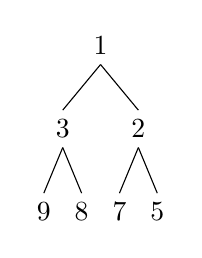
\begin{tikzpicture}
\Tree [.1 [.3 9 8 ] [.2 7 5 ] ]
\end{tikzpicture}
\caption{[1, 3, 2, 9, 8, 7, 5]}
\end{figure}

\begin{figure}[H]
\centering
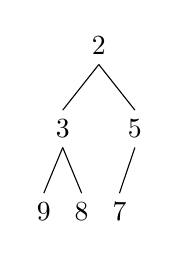
\begin{tikzpicture}
\Tree [.2 [.3 9 8 ] [.5 7 \edge[draw=none]; {} ] ]
\end{tikzpicture}
\caption{[2, 3, 5, 9, 8, 7]}
\end{figure}

\begin{figure}[H]
\centering
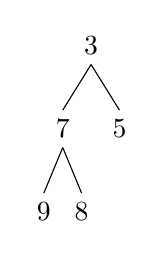
\begin{tikzpicture}
\Tree [.3 [.7 9 8 ] 5 ]
\end{tikzpicture}
\caption{[3, 7, 5, 9, 8]}
\end{figure}

\begin{figure}[H]
\centering
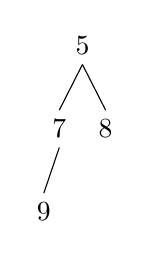
\begin{tikzpicture}
\Tree [.5 [.7 9 \edge[draw=none]; {} ] 8 ]
\end{tikzpicture}
\caption{[5, 7, 8, 9]}
\end{figure}

\noindent b.
\newline
Max Heap: [9, 8, 7, 3, 2, 5, 1]
\newline
1: [8, 3, 7, 1, 2, 5, 9]
\newline
2: [7, 3, 5, 1, 2, 8, 9]
\newline
3: [5, 3, 2, 1, 7, 8, 9]
\newline
4: [3, 1, 2, 5, 7, 8, 9]
\newline
5: [2, 1, 3, 5, 7, 8, 9]
\newline
6: [1, 2, 3, 5, 7, 8, 9]

\end{document}